\documentclass[12pt]{article}
%\usepackage{times}
\usepackage{cite}
\usepackage{graphicx}
\usepackage{url}
\setlength{\parskip}{1em}
\setlength{\parindent}{0em}
%this is a comment
\title{CS 361 \\ Design Implementation of System (DIS): \\ Digital Ghostwriter}
\author{Thomas Hollenberg (hollenbt), Zachary Thomas (thomasza),\\ Amar Raad (raadv), Jared Tence (tencej), \\  Zech DeCleene (decleenz)}
\date{February 10th, 2018}

\begin{document}
\maketitle
\newpage
\tableofcontents

\newpage

\section{UML Class Diagram}

\begin{figure}[ht]
  \centering
    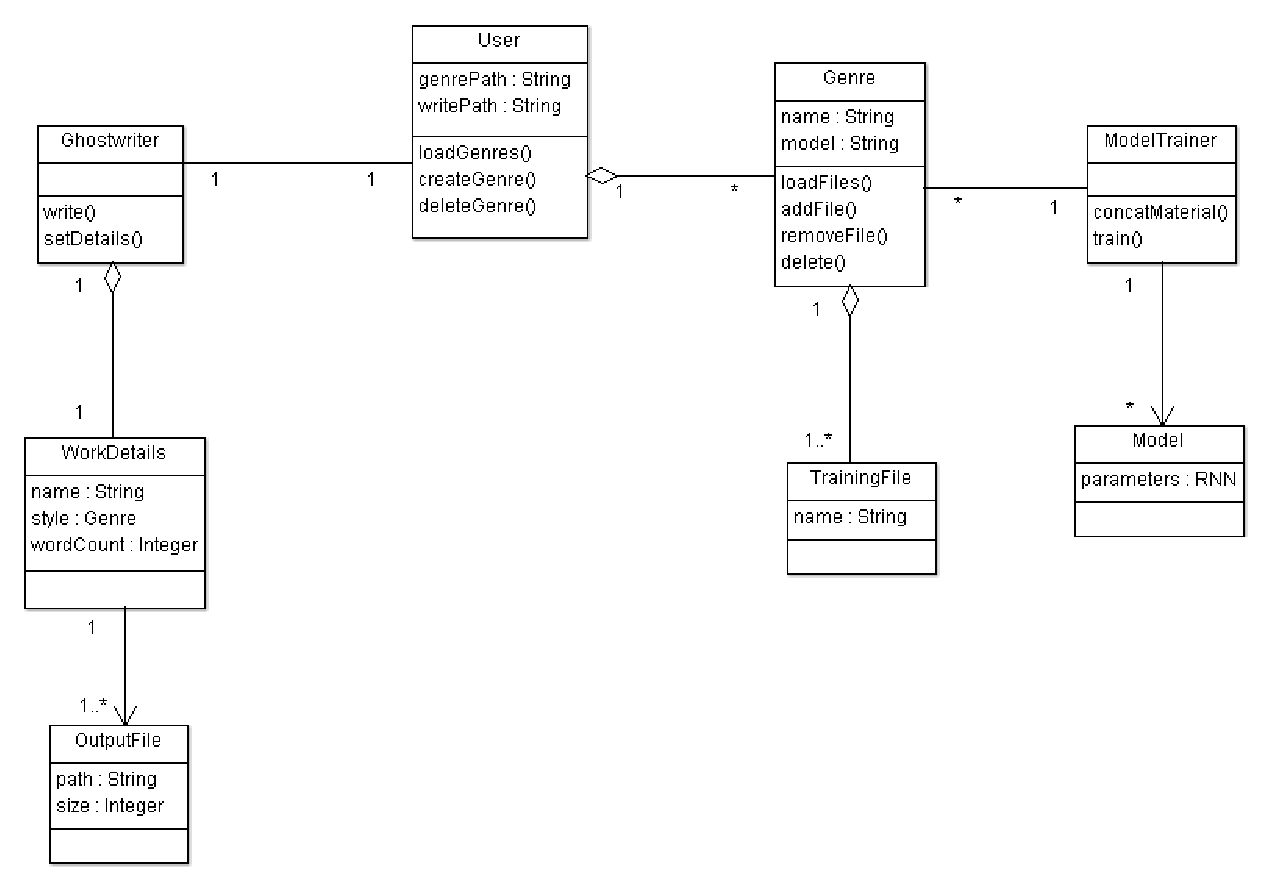
\includegraphics[scale=0.7]{ClassDiagram.eps}
\end{figure}

\newpage

\section{Packages}

We have three packages for our project, Word-rnn Tensorflow, the GUI interface, and the syntax checker.

Our Word-rnn Tensorflow package only relies on its text input from the GUI to generate a ghostwritten paper. Due to this single reliance, when fixing a flaw in our GUI interface it will not require us to edit the code within the Word-rnn Tensorflow package. Therefore Word-rnn Tensorflow has low coupling with the GUI interface. Tensorflow does have high cohesion, the algorithms and functions in the Word-rnn tensorflow are deeply connected, a small modification in a Tensorflow function, such as a policy change, will result in a vastly different output.

The GUI interface also has low coupling with the other packages. The GUI interface only feeds the Word-rnn Tenserflow package it's input and displays its output. A change in Tenserflow will result in a change of the saved output but not a change in the format of our GUI. Like Word-rnn Tensorflow it does have high coupling. Our GUI's pages rely on the previous pages inputs when the user selects the write option on our main page the GUI will use that previous input to display the written page instead of displaying the create genre page. Thus the code in our GUI interface package is very self-reliant making it very cohesive.

The Syntax Checker package like the other two also has low coupling and high cohesion. The Syntax Checker takes in the output of the Word-rnn Tensorflow package and sends it to the GUI which stores it. It acts as an intermediary between the two packages as it looks at the text and fixes any grammatical mistakes. Thus being very self-reliant. It is important for this package to be cohesive over having high coupling because this element won't be added until the GUI and Word-rnn Tensorflow are done making it important that we won't have to make dramatic changes as a result of implementing it.

\section{Design Patterns}

Our project is split into multiple design patterns based on the components we are using. We use the observer design pattern for our UI. We use the builder design pattern for our genre and ghostwriter components.

The observer design pattern is ideal for our UI, since the observer is able to watch for an object's state to change, it allows our software to react to user input as well as display pertinent feedback messages to the user, such as file write or read errors.

The builder design pattern is ideal for our genre machine learning component as it allows us to use learning material to produce models that are generated by our Model Trainer. The Model trainer has access to a directory filled with text files that it uses as training material which it concatenates into a single file and then produces a model file that is used by the Ghostwriter component. The builder design pattern favors such a step by step approach. 

The builder design pattern is also the ideal design pattern for the Ghostwriter component as it helps facilitate the creation of complex documents. The user simply selects a genre, word count, and a name for the text and based on a model previously generated by our Model Trainer the ghostwriter creates a text document using the given name that matches the users input. The builder design pattern allows us to encapsulate and hide the code used to implement this component. 

We have no need for complex iteration over data structures or decoding information so the Visitor and Decorator are ill suited for this project.
\newpage

\section{Interfaces and Contract}

We did not cover this particular topic in the class last week so we can ignore this section for this assignment. Approved by our instructor Ali Aburas.

\section{Exceptions and Handling}

Most exceptions that are likely to occur all have to do with file permissions and bad file paths.

First, if the user specifies a non-existant file path for the training material, or the file permissions to not allow it to be read, the model cannot be trained. The same is true if the specified model output file path is non-existant or the file permissions do not allow writing to that directory. These exceptions are related to genre creation. In these four cases, the exception handler should create a pop-up showing an error description and what the user needs to do to fix the issue (i.e. verify filepath, change permissions, etc.) before trying again, and focus should be returned to the genre-creation form.

Similar exceptions must be considered in the ghostwriting portion of the application. If the filepath to the model is non-existant or has incorrect file permissions, no output text can be generated. The same is true if the specified output file path is non-existant or has incorrect file permissions. In these four cases, the exception handler should create a pop-up showing an error description and what the user needs to do to fix the issue before trying again, and focus should be returned to the ghostwriting form.

Another class of potential exceptions have to do with incomplete form submission. For example, if the user attempts to create a new genre without a name or without supplying any training material. It may be possible to prevent the form from submitting and create an error message pop-up if some fields are missing or invalid. This would be the ideal way to handler this class of exception, because then the user's form progress would not be lost.

\section{Meeting Report }

\subsection{This week's progress:}
Made further progress on implementation of Digital Ghostwriter, completed Design Implementation of System phase and created a Google slides presentation.

\subsection{Goals for next week:}
Tuesday meeting at 3pm at Kelly to discuss and collaborate on our Digital Ghostwriter implementation. Practice and refine presentation.

\subsection{Contribution of team members:}
All team members gave feedback and worked on our assignment and presentation.

\subsection{Were customers able to meet with the team:}
Yes. Team including customers met to complete assignment and be present for our weekly meeting (2/11).


\end{document}
